\documentclass[dvipdfmx]{jsarticle}
\usepackage[T1]{fontenc}
\usepackage[dvipdfmx]{hyperref}
\usepackage{lmodern}
\usepackage{latexsym}
\usepackage{amsfonts}
\usepackage{amssymb}
\usepackage{mathtools}
\usepackage{amsthm}
\usepackage{multirow}
\usepackage{graphicx}
\usepackage{wrapfig}
\usepackage{here}
\usepackage{float}
\usepackage{ascmac}
\usepackage{url}

\title{Groceriesに関するR言語を使用した頻出パターン抽出及び相関ルール分析}
\author{文理学部情報科学科\\5419045 高林 秀}
\date{\today}

\begin{document}

\maketitle

\begin{abstract}
  本稿では、今年度データ科学2で学習した「頻出パターン抽出」及び「相関ルール分析」の手法を使用して、R言語のライブラリであるarulesに付属しているデータGroceriesを対象とした頻出パターン抽出、相関ルール分析を行うものである。

\end{abstract}

\section{目的}
本稿では実際に、R言語を使用しライブラリarules付属のデータであるGroceriesの頻出パターン抽出、相関ルール分析を行うことで、本年度データ科学2で学習した頻出パターン、相関ルール分析の手法への理解を深め、その定着を図ることを目的とする。また、1年次に学習したlatexを用いたPDF作成の復習も兼ねるものである。
\section{理論説明}
今回の実験で用いた、計算理論をそれぞれ説明する。
\subsection{バスケット分析}
初めに、頻出パターン抽出、相関ルール分析を説明する前に「バスケット分析」について説明する。\par
バスケット分析とは、データマイニングにおける代表的な手法の1つで、「顧客の購買記録をデータ化し分析を行うことで、顧客に共通するルールや傾向を導く」データ分析のことである。すなわち「一緒に買われやすい商品の組み合わせを見つける」ということである。\par
顧客の買い物データを分析しその結果を企業の販促活動などのマーケティングに関わる施策に適用するのが目的である。なお、バスケット分析はアソシエーション分析\footnote{データマイニングにおけるデータ間の関連性を見つける手法のこと。「もしAならばBである」といった法則を見つけ出し、主に購買記録などから顧客の購買行動の関連性を見つけ出すのに利用される。}の一つとされ、マーケットバスケット分析とも呼ばれる。\par
%%ここにバスケット分析の簡単な図説をのせる。
\subsection{頻出パターン・相関ルール分析の概要}
身の回りで頻出パターン抽出と相関ルール分析が使われている代表例としては、先に述べたバスケット分析をはじめ、オンラインショッピングサイト等のレコメンドシステム等が挙げられるだろう。頻出パターン抽出と相関ルール分析はこれらのシステムの基本的な原理である。この章では、頻出パターン抽出と相関ルール分析とはなにか概要を説明する。
\subsubsection{頻出パターン}
まず、頻出パターン(頻出アイテム集合)とはなにか説明する。頻出パターンとは「データベース中に高頻度で現れる組み合わせ、集合のこと」であり、頻出パターン抽出(頻出パターンマイニング)とはその集合を発見するための手法である。またこの集合のことを頻出アイテム集合と呼ぶ。頻出アイテム集合か、そうでないかを判断するための基準として後述する支持度(同時確率)と呼ばれる数値を計算し、その数値が、あらかじめ設定した閾値を超えるかどうかで判定する。頻出パターン抽出は「どの商品が一緒に購入されているか」を見るので、得られた結果は、商品の陳列場所の改善や、販促キャンペーン、店舗レイアウト等を考える際に利用することができる。\par
頻出パターン抽出は、後述する相関ルール問題の部分問題として広く認知されている。
\subsubsection{相関ルール}
次に、相関ルールとはなにか説明する。相関ルールとは「頻出パターン間の関係性」のことで、相関ルール分析はこの関係性すなわちルールを見つける目的で行われる。例えば、「あるアイテム集合$I1$が生起するとき、別のアイテム集合である$I2$も同時に生起する」といったようなものが相関ルールとなる。このとき、記号で「$\{I1\} \Rightarrow \{I2\}$」といった形で記述する。導いた相関ルールを評価する評価基準として、後述する確信度と呼ばれるものが存在する。具体的な計算法は後述するが、確信度とは一言で言えば「ルールの強さ」を示す指標で、左辺のアイテム集合が生起したときの右辺のアイテム集合の生起確率である。。加えて、支持度も利用される。相関ルールにおける評価指標としての支持度は「ルールの汎用性」を示すものとして利用される。\par
相関ルール抽出問題とは、あらかじめ設定する「最小支持度」「最小確信度」を閾値として、この閾値を超える相関ルールをデータベース上から見つけることを目的とした問題である。
\subsubsection{トランザクションデータベース}
頻出パターン・相関ルール分析は後述するように、形式的な定義のもとで、入力をうけその出力として頻出パターン・相関ルールを返す。このとき、入力として「トランザクションデータベース」が与えられる。\par
トランザクション(英名:transaction)とは、商取引、議事録、売買等の意味があり、情報処理用語としては一連の処理をひとつにまとめたものという意味をもつ。トランザクションデータベースとは、データの更新処理を一つにまとめているようなデータベースのことである。
\subsection{計算法}
この章では、実際に頻出パターンや相関ルールがどのように計算されているのかについて説明する。その前に、概要の部分で登場した「支持度」と「確信度(信頼度)」について説明する。以下の説明で使用する数式記号について、
\begin{center}
  \begin{gather*}
    D = {t_{1}, t_{2}, t_{3},..., t_{n}}:n個のトランザクションを含むデータベースD\\
    I = \cup_{t_{i}\in D}t_{i}:全アイテムの集合 \\
    t_{i} \subseteq I:i番目のトランザクション \\
    min\_sup(0 < min_sup \le 1):最小支持度 \\
    min\_conf(0 \le min_conf \le 1):最小確信度
  \end{gather*}
\end{center}
のように定義する。
\subsubsection{支持度(support)}
支持度とは「ルールの汎用性(一般性)の尺度」であり、集合$I1, I2$を例にしたベン図で示すと以下のようになる。
%%ここにベン図
%%提供:JSTデータマイニングコース:教材資料動画
これは、同時確率とみなすことができる。つまり、あるパターン$X$の支持度とは$X$中のアイテムが同時に出現する確率ということができる。これを式で示すと以下のようになる。
\begin{gather*}
  ※|a|:集合aの要素数\\
  sup_{D}(X) = \frac{|{t\in D|X\subseteq t}|}{|D|}
\end{gather*}
\begin{itemize}
  \item $t \in D$:アイテム集合Xを含むデータベース中のトランザクション
\end{itemize}
つまり、アイテム集合$X$の支持度は、$X$を含むトランザクションの割合、すなわち$X$中のアイテムがすべて出現するときの確率という意味で、その値は「$X$を含むデータベー上のトランザクション」を「データベース全体のトランザクション数」で除算した値である。\par
支持度が低いとは、そのパターンがごく少数の事例にのみ関係するパターンであり、いかに特徴的、すなわちその集合が他の部分集合を包含していて、少ないトランザクションに出現するということであり、データベースの一般的な傾向とはみなされていない、ということになる。反対に、支持度が高いとは、そのパターンがデータベース内で一般的、すなわち他の部分集合に包含されていて、多くのトランザクションに出現している、ということを意味している。
\subsubsection{確信度(confidence)}
確信度とは、「そのルールの確からしさの尺度」であり、データマイニングにおける相関ルールの重要度を示す指標である。別名、信頼度とも呼ばれる。\par
前章の部分でも述べたが、あるアイテム集合$I1$が生起するとき同時に$I2$も生起するという現象、ルールは$I1 \Rightarrow I2$で表記される。確信度とは、$I1 \Rightarrow I2$のルールの強さを示す指標と言える。$I1 \Rightarrow I2$の確信度を$conf_{D}(I1, I2)$と示すと、確信度は以下のように計算される。
\begin{gather*}
  conf_{D}(I1, I2) = \frac{|\{t \in D|I1 \subseteq t, I2 \subseteq t|\}}{\{|t \in D | I1 \subseteq t|\}}\\
  =\frac{|\{t \in D | (I1 \cup I2) \subseteq t\}|}{|\{t \in D | I1 \subseteq t\}|}
\end{gather*}
このとき、分母の式$|\{t \in D | I1 \subseteq t\}|$は$I1$の出現回数を示している。また分子の式$|\{t \in D | (I1 \cup I2) \subseteq t\}|$は、$I1, I2$の同時出現回数を示している。つまり確信度とは、$\frac{I1の出現回数}{I1とI2が同時に出現する回数}$の値ということになり、これは条件付き確率と同じになる。\par
確信度が低いときとは、そのルールが不正確であることを示している。反対に確信度が高いときとは、そのルールが正確なルールであることを示していることになる。
\subsubsection{頻出パターン抽出の計算法}
頻出パターン抽出の際は、入力としてトランザクションデータベースを受け取り、すべての頻出アイテム集合を出力する。
このとき、頻出パターン$F$は次の式で示すことができる。
\begin{gather*}
  F = \{X | X \subseteq I, X \neq \phi, sup_{D}(X) \ge min\_sup \}
\end{gather*}
\paragraph{頻出パターン抽出の計算量}
上記式で示すとおり、頻出パターンに選ばれた集合$X$の支持度は、予め定めた支持度の下限値すなわち最小支持度以上である必要がある。ということは、頻出パターンを見つけるには単純に、すべてのアイテム集合$$I$に属する、すべての部分集合の支持度を1つずつ計算していき、その値が最小支持度を超えるかどうか判定すれば良いことになる。しかし、現実の場合ではそうもいかない。ご存知の通り、我々が普段使うコンピュータの計算資源は無限ではなく有限である。したがって、あまりにも計算量が大きすぎる問題に関してはそもそも計算リソースが足らず、答えを求めることができない。\par
現実の現場(小売店やその他店舗)等で使用されるデータベースは膨大な数のデータを扱うことがほとんどである。そうなれば当然
すべてのアイテム集合$$I$の数も膨大である。以下に、すべてのアイテム集合$$I$の数を$|I|$としたときの冪集合\footnote{ある集合の部分集合全体の集合}の個数を示す。
\begin{gather*}
  冪集合の個数N = 2^{|I|}-1
\end{gather*}
\begin{table}[H]
  \begin{center}
    \caption{$|I|の値による冪集合の個数$}
    \begin{tabular}{|c|l|} \hline
      $|I|$ & 冪集合の個数 \\ \hline
      $|I| = 10$ & 1024 \\
      $|I| = 16$ & 65536 \\
      $|I| = 50$ & 約1.1京 ※$1京=10^{16}$\\
      $|I| = 100$ & 約1267穣 ※$1穣=10^{28}$\\
      $|I| = 200$ & 約1.6那由他 ※$1那由他=10^{60}, 一説では10^{72}$ \\ \hline
    \end{tabular}
    \label{hyo01}
  \end{center}
\end{table}
上記の表からも分かるとおり、現実の現場ではすべての冪集合を求めることは不可能に近い。したがってより効率的に頻出パターンを計算するアルゴリズム・手法が必要となる。そのような代表例として、後述する「バックトラック法」や「アプリオリアルゴリズム」が存在する。
\subsection{パターン空間について}
パターン空間とは、「考えうるすべてのアイテム集合を列挙したもの」である。すべてのアイテム集合$I$の部分集合、すなわち頻出パターンの候補を列挙し、その部分集合$P,Q$に対し$P \subseteq Q and |P| = |Q|-1$のとき線で結ぶ、という動作をする。このような操作で集合を図示、列挙すると「束(Lattice)」と呼ばれる、任意の2点間に上限と下限の存在する(半)順序集合ができあがる。すなわち、要素全てに共通する上限と下限が存在することを意味する。アイテム集合$I$の冪集合を対象にすると、下図に示すとおり上限は空集合$\{\phi\}$、下限は$I$となる。
%%ここにパターン空間の例を図示:教材資料1−16
\paragraph{支持度の逆単調性}
アイテム集合$P$とその部分集合$Q$、$P \subseteq Q$であるとき、$P$の支持度はその部分集合$Q$の支持度以上になることを「支持度の逆単調性」と呼ぶ。
\begin{gather*}
  sup_{D}(P) \geq sup_{D}(Q)
\end{gather*}
このことから次のことが導き出せる。
\begin{enumerate}
  \item $P \subseteq Q$であるとき$sup_{D}(P) \geq sup_{D}(Q)$
  \item $P$の支持度が最小支持度未満であるとき、$P$のすべての上位集合の支持度は最小支持度未満になる。
  \item 上記より、最小支持度未満となる集合の上位集合は必ず頻出パターンになることはない。よって計算する必要がなくなる。
  \begin{gather*}
    sup_{D}(P) < min\_sup \to \forall Q_{\supseteq P}[sup_{D}(Q) < min\_sup]\\
    \forall Q_{\supseteq P}:QはPの上位集合
  \end{gather*}
\end{enumerate}
頻出パターンの発見は、言い換えると考えうるパターン空間から、最小支持度以上を満たす頻出アイテム集合を探すということになる。ただし先に述べたように、すべてを探索し切るのは困難なので前述した「支持度に関する逆単調性」を利用して探索範囲を限定(枝刈り)することが求められる。
\paragraph{(補足)深さ優先探索・幅優先探索}
木構造をとるデータ構造におけるデータの探索手法として深さ優先探索(depth-first search)と幅優先探索(breath-first search)が存在する。\par
深さ優先探索とは下図に示すとおり、探索の順序を「木の深さ(レベル)を大きくするように」探索する手法で、進めるところまで進んでこれ以上進めなくなったら一度上の深さまで戻ってまた探索をする、といったような動作をする。\par
反対に幅優先探索は、探索の順序を「同じ深さに属するデータから順番に見るように」探索する手法で、探索の出発点から横に近い順番で探索をする、といったような動作をする。
\begin{figure}[H]
  \centering
  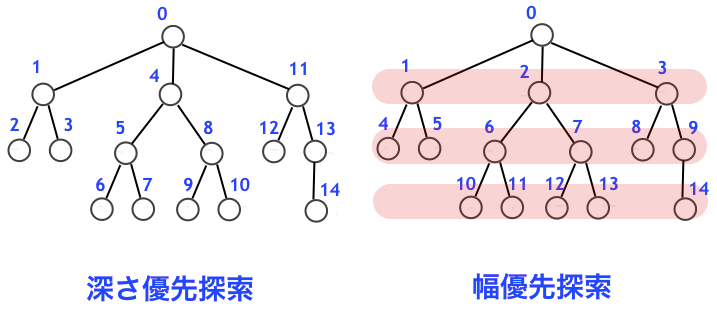
\includegraphics[scale=0.4]{images/hosoku.png}
  \caption{深さ優先探索と幅優先探索}
  出典:\url{https://qiita.com/drken/items/4a7869c5e304883f539b}
\end{figure}
\begin{table}[H]
  \begin{center}
    \caption{深さ優先探索と幅優先探索の相違点}
    \begin{tabular}{|c|c|} \hline
      深さ優先探索 & 幅優先探索 \\ \hline
      & \\
      & \\
      & \\ \hline
    \end{tabular}
    \label{hyo02}
  \end{center}
\end{table}
\subsection{バックトラック法}
前述したように、パターン空間から考えうるすべての冪集合の支持度を計算し頻出アイテム集合を決定するのは計算量と効率の面から非現実的である。したがって、より効率の良い計算方法のとして「バックトラック法」と「アプリオリアルゴリズム」を先に例示した。ここではバックトラック法についての具体的な説明を行う。\par
まず、バックトラック法とはなにか。バックトラック法とは「考えうるすべてパターンを系統的に探索し答えを得る」手法で、探索時の頻出アイテム集合の候補数をできるだけ少なくすることで探索時の効率を上げるというものである。バックトラック法は支持度の逆単調性を利用して探索時の頻出アイテム集合の候補数を限定している。そのため、すべてのアイテム集合を探索しないとはいえ頻出アイテム集合を逃すことはない。\par
%%ここに図示
バックトラック法は、パターン空間内の集合に「親」を設定することによってグラフから木構造へ変形する。このとき、親とは包含するアイテム集合(そのアイテム集合のパターン空間における1つ下にあるアイテム集合)から「最大のアイテムを削除した集合」ということなる。また、親の子は親の集合を得る逆の操作をすれば良いので、その集合の要素より大きなアイテムを1つ追加した集合となる。\par
この親子関係が結ばれる集合同士を線で結ぶとき、あるアイテム集合の親は必ず1つに定まる。したがって、そのアイテム集合は自身の親からのみ探索することができるので入力が1つに決まる。これを図示すると下図のようになり、木構造が出来上がる。このときの木構造を「集合列挙木」と呼ぶ。\par
%%ここに図示
上図からも分かるとおり、各子集合は親集合からのみ探索することができるので探索時に重複することはない。バックトラック法はこの集合列挙木を作成しながら、アイテム集合の支持度を計算し、最小支持度以下ならば、支持度の逆単調性より、それより深いアイテム集合の探索を打ち切る、すなわち枝刈りを行うことで探索の効率を高めている。このとき、あるアイテム集合の支持度が最小支持度未満であるときそれより先のアイテム集合の探索を打ち切り、親に戻って(バックトラック)また探索をするのでバックトラック法は、深さ優先探索であると言うことができる。\par
以下にバックトラック法の擬似的なpythonコードを示す。
\begin{align*}
  &def backtrack(D, min\_sup): \\
  & I = \cup_{t \in D}t \#全アイテム集合を取得しIに代入\\
  & dfs(\phi, I, D, min\_sup) \#深さ優先探索(depth-first-search) \\
\end{align*}
\begin{align*}
  &def dfs(P, I, D, min\_sup): \\
  & for i in I: \\
  &  Q.append(P\cup i) \#子アイテム集合Qにアイテムiを追加 \\
  &  if sup_{D}(Q) \geq min\_sup: \\
  &   print(Q) \#Qを出力 \\
  &   dfs(Q, I, D, min\_sup) \#再帰呼び出し\\
  &  else: \\
  &   pass \\
\end{align*}
\subsection{アプリオリアルゴリズム}
次に挙げられる方法として、「アプリオリアルゴリズム」が存在する。アプリオリアルゴリズムはバックトラック法とは異なり、支持度の逆単調性を利用した幅優先探索である。バックトラック法では、親すなわち一つの部分集合の支持度のみを計算していたが、アプリオリアルゴリズムではすべての部分集合に対して支持度を計算する。したがって、探索の仕方が階層的、横に進むようになることから幅優先探索と言える。\par
アプリオリアルゴリズムには大きく分けて以下の2ステップがある。
\begin{itemize}
  \item ジョインステップ(Join Step)
  \item プルーンステップ(Prune Step)
\end{itemize}
このアルゴリズムでは、頻出アイテム集合を、集合の要素数の大きい方から順番に1~$$K$まで求めていく。サイズ$K$の頻出アイテム集合(以下$K-itemset$)を求めるため1つ要素数が大きい$K+1-itemset$を利用する。
\paragraph{ジョインステップ}ジョインステップは、結合ステップとも呼ばれる。\par
このステップでは、2つの$K-itemset$を利用して$K+1-itemset$の候補を生成する。
\begin{gather*}
  C_{K+1}^{join} = \{X \cup Y\ |
  \left.
  \begin{array}{l}
    X \in L_{K}, Y \in L_{K} \\
    X \setminus \{tail(X)\} = Y \setminus \{tail(Y)\}, \\
    tail(X) < tail(Y) \\
  \end{array}
  \right.
\end{gather*}

\subsection{相関ルール抽出の計算法}
\subsection{相関ルール分析の評価基準}

\section{計算機実験}
\subsection{実験準備}
  \subsubsection{実験環境}
  今回の実験は仮想マシン上でR言語を起動し行った。下記に実験時の環境を示す。
  \begin{itemize}
    \item ホストOS:Window10 Home Ver.20H2
    \item 仮想OS:Ubuntu 20.04.2 LTS
    \item CPU:Intel(R)Core(TM)i7-9700K @ 3.6GHz
    \item GPU:Nvidia Geforce RTX2070 OC @ 8GB
    \item ホストRAM:16GB
    \item 仮想RAM:4GB
  \end{itemize}
\subsubsection{実験データ}
\subsubsection{R言語での頻出パターン・相関ルール分析の手法}
\subsection{実験結果}
\subsection{結果の説明}

\section{考察}
\section{まとめ}

\begin{thebibliography}{99}
  \bibitem 冪集合について:\url{https://mathlandscape.com/power-set/#:~:text=%E4%B8%80%E8%A8%80%E3%81%A7%E3%81%84%E3%81%86%E3%81%A8,%E3%81%AE%E9%9B%86%E5%90%88%E3%82%92%E6%8C%87%E3%81%97%E3%81%BE%E3%81%99%E3%80%82}
\end{thebibliography}
\end{document}
